\documentclass[parskip=full, 12pt, oneside]{scrbook}

\usepackage[utf8]{inputenc} % use utf8 file encoding for TeX sources
\usepackage[T1]{fontenc} % avoid garbled Unicode text in pdf
\usepackage[english]{babel} % english hyphenation, quotes, etc
\usepackage[hidelinks]{hyperref} % detailed hyperlink/pdf configuration
\usepackage{csquotes}
\usepackage{authblk}
\usepackage{enumitem}
\usepackage{graphicx} %%provides the  \includegraphics macro
\usepackage{float} %%provides the H directive to force position of figures (\begin{figure}[H])
\usepackage[numberedsection,nonumberlist,toc,section=chapter]{glossaries}     % provides glossary commands
\usepackage{scrhack} %%make above float package compatible with komascript
\usepackage{ifthenx}
\usepackage{intcalc}
\hypersetup{ % `texdoc hyperref` for options
	pdftitle={Functional Specifications},
	bookmarks=true,
}

\makenoidxglossaries

% Configure Title Page Layout
\subject{Karlsruhe Institute of Technology}
\author{
	\textit{Irma Suppes, Karl Rubel, } \\ 
	\textit{Mingyi Li, Niklas Bülow, Sönke Jendral }
}
\title{MORR \\ (Medical Online Research Recorder)}
\subtitle{PSE-Project \\ Functional Specification Document}
\publishers{Supervisors: \\ \textit{Paula Breitling, Dr. Till Riedel, Tobias Röddiger}}

\chapter{Glossary}
\label{ch:glossary}

\begin{document}

\newcommand{\requirementscope}[2]{\newcounter{counter#1}\expandafter\def\csname #2\endcsname{\addtocounter{counter#1}{10}\item[#1\arabic{counter#1}\phantomsection\label{#1\arabic{counter#1}}]}}
\newcommand{\specref}[1]{\hyperref[#1]{#1}}

\maketitle

\chapter*{Document Version History}
\label{ch:versionhistory}
\begin{table}[h]
\begin{tabular}{lll}
\textbf{Revision} & \textbf{Date} & \textbf{Description}              \\
\hline
1.0.0             & 13.12.2019    & Creation and release of document. \\
\hline
1.1.0			  & 14.02.2020	  & Update software-design: \\
&& Update BrowserExtension Shared section\\
&& (Update EventType enum and serialize method)\\
&& Update BrowserExtension Background section\\
&& (Update methods of BackgroundScript and ICommunicationInterface)\\
&& Update BrowserExtension Listeners section\\
&& (Update factory methods)\\
&& Update BrowserExtension Content section\\
&& (Update method signature in DOMEventFactory)\\
&& Update ClipboardModule section\\
&& (Update producers methods, add new ClipboardEvents)\\
&& Update KeyboardModule section\\
&& (Update producers methods, update attributes in KeyboardInteractEvent)\\
&& Update MouseModule section\\
&& (Update producers methods, add MouseModuleConfiguration,\\
&& update attributes in mouse events)\\
&& Update WebBrowserModule section\\
&& (Update producers methods, add WebBrowserModuleConfiguration,\\
&& add classes for communication with WebExtension,\\
&& add WebBrowserProducer abstract class)\\
&& Update WindowManagementModule section\\
&& (Update producers methods)\\

\end{tabular}
\end{table}% History of document versions
\tableofcontents
\chapter{Introduction}
\label{ch:introduction}	% Introduction
\chapter{Definition of Goals}
\label{ch:goals}

\requirementscope{MC}{mspec}
\requirementscope{OC}{ospec}
\requirementscope{DC}{dlspec}

The purpose of this project is to create an application which records the online research process of \glspl{user}. The focus of the application is to collect data and make it available to \glspl{scientist}. This chapter gives an overview of the functionality of the product. It describes the informal requirements and is used to establish a context for the technical requirements specification in the following chapters.


\section{Mandatory Criteria}

\begin{itemize}
	\mspec{Data recording}{\Gls{user} interactions during the online research must be recorded.}
	\mspec{\Gls{user} controllability}{The recording \gls{session} is controlled by the \gls{user}. It must be started and stopped by the \gls{user}.}
	\mspec{Start notification}{Start notification informs the \gls{user} about the start of the recording \gls{session} and must be displayed to the \gls{user} before the start of the recording \gls{session}.}
	\mspec{\Gls{user} awareness}{A \gls{user} must be aware of the recording process at any time during the \gls{session}.}
	\mspec{Confirmation of the saving of the recorded data}{A \gls{user} is asked to confirm if the recorded \gls{session} is to be saved.}
	\mspec{Past recording \glspl{session}}{A \gls{user} must be able to view the recordings of the past \glspl{session}.}
	\mspec{Data provisioning}{A \gls{scientist} must be able to extract the recorded data.}
\end{itemize}

\addtocounter{section}{1} %%removed optional criteria
\section{Delimiting Criteria}

\begin{itemize}
	\dlspec{Data interpretation}{The application does not interpret the recorded data.}
	\dlspec{Spying on the \gls{user}}{The application does not secretly monitor and gather information about the \gls{user}.}
\end{itemize}			% Definition of Goals
\chapter{Project Scope}
\label{ch:scope}

\section{Scope}
The application is used to record cancer or genetic disorder related researches conducted by a medical staff member and gather data for \glspl{scientist}.
\section{Target Audience}
The application is aimed at two major audiences:
\begin{enumerate}
    \item Medical staff members who conduct cancer or genetic disorder related researches in certain online databases.
    \item \Glspl{scientist} who make use of the gathered data.
\end{enumerate}
\section{Operating Conditions}
The application will be used in an office or at home during research.			% Application Scope
\chapter{Project Environment}
\label{ch:environment}

The product runs on a personal computer.

\section{Software}
\begin{itemize}
\item[] Operating System: Microsoft Windows 10 (minimum build: 1803)

\item[] Development Tools:
	\begin{itemize}
	\item Programming Languages: \\C\# (Core Application), JavaScript (WebExtensions)
	\item Integrated Development Environment (IDE): Microsoft Visual Studio 2019
	\item Documents: LaTeX
	\item Version Control: Git (GitLab)
	\end{itemize}
\end{itemize}
\section{Hardware}

The application runs on personal computers with stable internet connection and average or better performance.	% Project Environment
\chapter{Functional Specifications}
\label{ch:func}

\newcounter{counterFS}
\newcommand{\internalspec}[5]
{
    \item[FS\arabic{counterFS}\phantomsection\label{FS\arabic{counterFS}}]
    \begin{itemize}[noitemsep]
        \item[]{\textbf{#1}} %title
        \item[]{Actor: #2}
        \item[]{Precondition: #3}
        \item[]{Action: #4}
        \item[]{Postcondition: #5}
    \end{itemize}
}
\newcommand{\fspec}[6][]{\ifthenelse{\equal{#1}{}}{\setcounter{counterFS}{\intcalcAdd{\value{counterFS}}{\intcalcSub{10}{\intcalcMod{\value{counterFS}}{10}}}}}{\setcounter{counterFS}{#1}}\internalspec{#2}{#3}{#4}{#5}{#6}}
\newcommand{\fsubspec}[5]{\stepcounter{counterFS}\internalspec{#1}{#2}{#3}{#4}{#5}}

%%commonly used post-conditions
\newcommand{\sessionactive}{A \gls{session} is currently being recorded.}
\newcommand{\sessioninactive}{No \gls{session} is currently being recorded.}
\newcommand{\sessionsavail}{One or more sessions have been recorded and not deleted.}
\newcommand{\applaunched}{The application is running.}
\newcommand{\configvalid}{The configuration file is valid.}
\newcommand{\configinvalid}{The configuration file is invalid.}
This chapter is meant to organize and describe the specifications that dictate the way the application functions for different actors.

\section{High-level specification}
\label{sec:func_highlevel}
The user interface components mentioned in this section are specified in \ref{sec:uispec}.
\begin{itemize}
    \fspec{Identifiable \glspl{session}}{\Gls{user}}{\applaunched{} \configvalid{}}{When the user starts a \gls{session}-recording by pressing the ``Start Recording''-button, a unique session-ID gets created.}{The recording-managing component holds a session-ID which all \glspl{event} recorded during the current \gls{session} will get associated with.}
    \fspec{Event timings}{\Gls{user}}{\sessionactive}{When the user triggers an event specified in chapter \ref{ch:data}, the respective \gls{module} (see \ref{sec:modules}) generates a data-structure (as defined in \ref{sec:events}) associated with the event and adds the timestamp to it.}{The data structure associated with the event is sent to the data-managing component and contains a timestamp describing its time of occurence.}
    \fspec{Event types}{\Gls{user}}{\sessionactive}{When the user triggers an event specified in chapter \ref{ch:data}, the respective module (see \ref{sec:modules}) generates a data-structure (as defined in \ref{sec:events}) associated with the event and adds the event-type to it.}{The data structure associated with the event is sent to the data-managing component and contains a field describing its \gls{event}-type.}
    \fspec{Event processing}{\Gls{user}}{\sessionactive}{When the user triggers an event specified in chapter \ref{ch:data}, the data structure corresponding to this event is processed and filtered by \glspl{module} (see \ref{sec:modules} and \ref{sec:sysarchitecture}). If the configuration does not specify to discard the event, the event data structure is sent to the data-managing component by the respective module.}{The event data structure is either sent to the data-managing component for serialization or deleted based on a configured rule.}
    \fspec{Configurability}{\Gls{admin}}{\sessioninactive}{An \gls{admin} opens the configuration file and adds/modifies/removes rules affecting some of the configurable behavior.}{The configuration-managing component will use the configuration as specified in the changed configuration file the next time the application is launched.}
    \begin{itemize}
    \fsubspec{Configuring active modules}{\Gls{admin}}{\sessioninactive}{An \gls{admin} opens the configuration file and changes the \glspl{module} the application is allowed to use.}{The module-managing component will manage the \glspl{module} as specified in the changed configuration file the next time the application is launched.}
    \fsubspec{Configuring video recording}{\Gls{admin}}{\sessioninactive}{An \gls{admin} opens the configuration file and changes the framerate, bitrate or resolution of the recorded videostream.}{The video-recording-managing component will record the videostream as specified in the changed configuration file the next time the application is launched.}
    \fsubspec{Configuring audio recording}{\Gls{admin}}{\sessioninactive}{An \gls{admin} opens the configuration file and enables or disables the recording of audio.}{The audio-recording-managing component will record or not record audio as specified in the changed configuration file the next time the application is launched.}
    \fsubspec{Configuring saving path}{\Gls{admin}}{\sessioninactive}{An \gls{admin} opens the configuration file and changes the system path where the recording of the current \gls{user} will be stored.}{The recording-managing component will store the recordings at the location as specified in the changed configuration file the next time the application is launched.}
    \end{itemize}
    \fspec{Error-detection}{\Gls{user}}{\configinvalid}{The \gls{user} starts the application. The configuration-managing component checks the configuration file and detects syntactic errors, therefore the application interrupts the startup procedure.}{The application has not regularly started and is therefore not ready for recording. For UI details, see \hyperref[sec:uispec]{Error dialogue}.}
    \fspec{\Gls{user} controllability (start)}{\Gls{user}}{\applaunched{} \sessioninactive}{The \gls{user} clicks on the button labeled ``Start Recording''. The recording-managing component starts a new \gls{session}-recording once the information dialogue (see \specref{FS80}) is confirmed by the \gls{user}.}{\sessionactive}
    \fspec{\Gls{user} instruction}{\Gls{user}}{\applaunched{} \sessioninactive{} \configvalid}{The \gls{user} clicks on the button labeled ``Start Recording''. The user-interface-managing component opens an information dialogue.}{A dialogue is being displayed, advising the \gls{user} not to enter any personal or confidential business information.}
    \fspec{\Gls{user} controllability (stop)}{\Gls{user}}{\sessionactive}{The \gls{user} clicks on the button labeled ``Stop Recording''. The recording-managing component will stop the current \gls{session}-recording.}{\sessioninactive{} The user-interface-managing component shows the save-dialogue to the \gls{user}, providing the options to store or discard the recorded session. For UI details, see \hyperref[sec:uispec]{Save dialogue}.} %%TODO: link UI
    \fspec{\Gls{user} controllability (quit)}{\Gls{user}}{\applaunched{} \sessioninactive}{The user chooses the ``Quit'' option. The application terminates.}{The application is no longer running.}
    \fspec{Quit while recording}{\Gls{user}}{\applaunched{} \sessionactive}{The user chooses the ``Quit'' option while a session is being recorded. The user-interface-managing-component opens the save-dialogue.}{The save-dialogue is shown to the \gls{user}. The application terminates immediately if the \gls{user} decided to discard the recording or terminates after the recording has been saved by the recording-managing component if the \gls{user} decided to save the recording.}
    \fspec{Save prompt}{\Gls{user}}{A \gls{session}-recording has been stopped and the save-dialogue is displayed.}{The user chooses whether to save or discard the recorded session.}{If the user chose to save the recording, the recording is stored by the recording-managing component at the location specified in the configuration file. If the user chose the discard-option, the recording is not stored.}
    \fspec{\Gls{user} reviewability}{\Gls{user}}{\sessionsavail}{A \gls{user} clicks on the ``Open recordings folder'' button. The user-interface-managing component opens the recordings folder in the Windows File Explorer, displaying the files in which this \gls{user}'s past recordings have been stored.}{The folder containing the user's recordings is opened in the Windows File Explorer. The \gls{user} can view the videostream contained in these files by opening them with a compatible video-player, e.g. Windows Media Player.}
\end{itemize}

\section{Core application specification}
\label{sec:func_core}
The core application has to cover the following responsibilities:
\begin{itemize}
    \fspec[200]{Videostream recording}{\Gls{user}}{\sessionactive}{While a session is being recorded, the video-recording-managing component constantly captures the \gls{device}'s primary screen's content into a videostream which the recording-managing component then serializes. The \gls{videostream} forms the basis for every recording.}{The \gls{session} recording contains a \gls{videostream} containing the \gls{device}'s primary screen's content.}
    \fspec{\hyperref[sec:system-modules]{System module} invocation}{\Gls{user}}{\applaunched}{The \gls{user} clicks the ``Start recording'' button. The system-module-managing component invokes the necessary \hyperref[sec:system-modules]{system modules} according to the configuration.}{All \hyperref[sec:system-modules]{system modules} that should be active according to the configuration are active and listening for their respective \glspl{event}.}
    \fspec{\hyperref[sec:system-modules]{System module} configuration}{\Gls{user}}{\configvalid}{The \gls{user} starts the application. The system-module-managing component configures the \hyperref[sec:system-modules]{system modules} according to the configuration.}{The \hyperref[sec:system-modules]{system modules} are configured according to the configuration and the application is ready for recording.}
    \fspec{\hyperref[sec:on-demand-modules]{On-demand module} registration}{\Gls{user}}{\sessionactive}{The \gls{user} starts an application (e.g. a \gls{browser}) which contains an \hyperref[sec:on-demand-modules]{on-demand module}. The \hyperref[sec:on-demand-modules]{on-demand module} notifies the on-demand-module-managing component about its availability. The on-demand-module managing component reacts by opening a communication port to the \hyperref[sec:on-demand-modules]{on-demand module} to allow for reception of event-data. It also configures the \hyperref[sec:on-demand-modules]{on-demand module} according to the configuration.}{The \hyperref[sec:on-demand-modules]{on-demand module} is ready to send filled-in \glspl{event} to the data-managing component.}
    \fspec{\hyperref[sec:on-demand-modules]{On-demand module} initial registration}{\Gls{user}}{\applaunched{} An application containing an \hyperref[sec:on-demand-modules]{On-demand module} is already running.}{The \gls{user} clicks on the button labeled ``Start Recording''. The on-demand-module managing component registers the available \hyperref[sec:on-demand-modules]{On-demand module} and reacts by opening a communication port to the \hyperref[sec:on-demand-modules]{on-demand-module} to allow for reception of event-data. It also configures the \hyperref[sec:on-demand-modules]{on-demand module} according to the configuration.}{The \hyperref[sec:on-demand-modules]{on-demand module} is ready to send filled-in \glspl{event} to the data-managing component.}
    \fspec{Data serialization}{\Gls{user}}{\sessionactive}{The \gls{user} triggers an event which is noticed by a \gls{module}. The \gls{module} sends the filled-in event to the data-managing component. The data-managing component collects events from multiple modules and the recording-managing component stores them in the same file (see \ref{sec:session_recordings}).}{The event-data received from all active \glspl{module} is written to the same file.}
    \fspec{Combinability of \glspl{module}}{\Gls{user}}{\configvalid{} All modules required by the configuration are installed.}{The \gls{user} starts the application and starts a \gls{session}-recording. The module-managing component sets up the internal processing-pipeline described in \ref{sec:sysarchitecture} in such a way that modules that receive events as input are connected to those that generate events as output and the modules adhere to the configuration.}{The application is ready to process the \glspl{event} in the pipeline as configured.}
    \fspec{Context management}{\Gls{user}}{\sessionactive}{After interacting with an application \textbf{A}, the \gls{user} starts interacting with another application \textbf{B}. The context-managing component registers this change (see \ref{sec:context}) and informs its modules where necessary.}{The context-managing component holds information on the current context and the modules that need to be informed about changes to the context have been informed.}
\end{itemize}

\section{User interface specification}
\label{sec:uispec}
\begin{itemize}
    \fspec[300]{Recording indicator}{\Gls{user}}{\applaunched{} \sessioninactive{} \configvalid}{The \gls{user} clicks on the button labeled ``Start Recording''. The user-interface-managing component will start showing a yellow border along the screen edges.}{A yellow border is being drawn along the screen edges as long as the recording is active.}
    \fspec{Error dialogue}{\Gls{user}}{\configinvalid}{The \gls{user} starts the application. The configuration-managing component will detect syntactic errors in the configuration file and the user-interface-managing component will display an error-message.}{An error-dialogue is shown, informing that the current configuration is invalid. When the user clicks the ``OK'' button shown in this dialogue, the application will terminate.}
    \fspec{Save dialogue}{\Gls{user}}{\sessionactive}{The user stops the recording by pressing the ``Stop Recording'' button or the ``Quit'' button. The user-interface-managing component opens a new dialogue.}{A dialogue window is shown to the \gls{user}, providing the options ``Save recording'' and ``Discard recording''.}
    \fspec{Event-Data extraction}{\Gls{scientist}}{\sessionsavail}{A \gls{scientist} starts the supplied command-line-tool and supplies the paths of one or multiple recordings as well as an output path as parameters. The tool will start extracting the stored event-data from the recording.}{The event-data has been extracted from the specified recordings and stored in CSV-format (comma separated values) at the location specified as output path. The recordings specified as input files have not been altered.}
    \fspec{Tray-Icon}{\Gls{user}}{\configvalid}{The user starts the application. The user-interface-managing component adds a new icon to the tray, indicating that the software has been launched successfully.}{An additional icon is shown in the system tray.}
    \fspec{Tray-Menu}{\Gls{user}}{\applaunched}{The user clicks on the tray-icon. The user-interface-managing component shows a menu providing the following options:
    \begin{itemize}
    \item ``Start recording'' or ``Stop recording'' (based on whether a session is already being recorded)
    \item ``Open recordings directory''
    \item ``Quit''
    \end{itemize}}{A small menu is shown above the tray icon, providing above options.}
\end{itemize}

\section{Per-module specification}
\label{sec:modules}
This section discusses the default \glspl{module} which will be available and ship with the application at release in order to fulfill the mandatory requirements.

\subsection{System modules}
\label{sec:system-modules}

System modules are \glspl{module} which communicate with the operating system. They are invoked as soon as a \gls{session}-recording is started and only terminate at the end of a recording. All system \glspl{module} are \hyperref[collecting-module]{collecting modules} as specified in \ref{sec:module-types}.

\subsubsection{Window-management module}

\begin{itemize}
    \fspec[400]{Window management events}{\Gls{user}}{\sessionactive}{When the \gls{user} performs one of the following window interactions, a window \gls{event} (as defined in \specref{D310}) gets created by this \gls{module} and sent to the data-managing component.}{The data-managing component received a filled-in window \gls{event}.}
    \begin{itemize}
    \fsubspec{Focusing a window}{\Gls{user}}{\sessionactive}{The \gls{user} focuses a window. The module creates a focus-window \gls{event} (as defined in \specref{D311}) and sends it to the data-managing component.}{The data-managing component received a filled-in focus-window \gls{event}.}
    \fsubspec{Moving a window}{\Gls{user}}{\sessionactive}{The \gls{user} moves a window. The module creates a move-window \gls{event} (as defined in \specref{D312}) and sends it to the data-managing component.}{The data-managing component received a filled-in move-window \gls{event}.}
    \fsubspec{Resizing a window}{\Gls{user}}{\sessionactive}{The \gls{user} modifies the size of a window. The module creates a resize-window \gls{event} (as defined in \specref{D313}) and sends it to the data-managing component.}{The data-managing component received a filled-in resize-window \gls{event}.}
    \fsubspec{Minimizing/Maximizing/Restoring a window}{\Gls{user}}{\sessionactive}{The \gls{user} minimizes, maximizes or restores a window. The module creates a minimize-window/maximize-window/restore-window \gls{event} (as defined in \specref{D314}) and sends it to the data-managing component.}{The data-managing component received a filled-in minimize-window/maximize-window/restore-window \gls{event}.}
    \end{itemize}
\end{itemize}

\subsubsection{Mouse module}

\begin{itemize}
    \fspec{Mouse interaction events}{\Gls{user}}{\sessionactive}{When the \gls{user} performs one of the following mouse inputs, a specialized mouse \gls{event} gets created by this \gls{module} and sent to the data-managing component.}{The data-managing component received a filled-in mouse \gls{event}.}
    \begin{itemize}
    \fsubspec{Mouse Click}{\Gls{user}}{\sessionactive}{The \gls{user} presses/releases the left/right/middle mouse button. The module creates a press/release left/right/middle mouse-button \gls{event} (as defined in \specref{D320}) and sends it to the data-managing component.}{The data-managing component received a filled-in press/release left/right/middle mouse-button \gls{event}.}
    \fsubspec{Scroll Wheel}{\Gls{user}}{\sessionactive}{The \gls{user} scrolls the mouse-wheel. The module creates a scroll mouse-wheel \gls{event} (as defined in \specref{D321}) and sends it to the data-managing component.}{The data-managing component received a filled-in scroll mouse-wheel \gls{event}.}
    \fsubspec{Mouse Movement}{\Gls{user}}{\sessionactive}{The \gls{user} moves the mouse. The module creates a mouse-movement \gls{event} (as defined in \specref{D322}) and sends it to the data-managing component.}{The data-managing component received a filled-in mouse-movement \gls{event}.}
    \end{itemize}
\end{itemize}

\subsubsection{Keyboard module}

\begin{itemize}
    \fspec{Keyboard interaction events}{\Gls{user}}{\sessionactive}{When the \gls{user} performs one of the following keyboard inputs, a specialized keyboard \gls{event} gets created by this \gls{module} and sent to the data-managing component.}{The data-managing component received a filled-in keyboard \gls{event}.}
    \begin{itemize}
    \fsubspec{Releasing/Pressing a key}{\Gls{user}}{\sessionactive}{The \gls{user} presses/releases a key. The module creates a press/release keyboard-key \gls{event} (as defined in \specref{D330}) and sends it to the data-managing component.}{The data-managing component received a filled-in press/release keyboard-key \gls{event}.}
    \end{itemize}
\end{itemize}

\subsubsection{Clipboard module}

\begin{itemize}
    \fspec{Clipboard events}{\Gls{user}}{\sessionactive}{When the \gls{user} performs one of the following clipboard-interactions, a specialized clipboard \gls{event} gets created by this \gls{module} and sent to the data-managing component.}{The data-managing component received a filled-in clipboard \gls{event}.}
    \begin{itemize}
    \fsubspec{Copying to the clipboard}{\Gls{user}}{\sessionactive}{The \gls{user} copies data to the clipboard. The module creates a clipboard-copy \gls{event} (as defined in \specref{D340}) and sends it to the data-managing component.}{The data-managing component received a filled-in clipboard-copy \gls{event}.}
    \fsubspec{Pasting from the clipboard}{\Gls{user}}{\sessionactive}{The \gls{user} pastes data from the clipboard. The module creates a clipboard-paste \gls{event} (as defined in \specref{D340}) and sends it to the data-managing component.}{The data-managing component received a filled-in clipboard-paste \gls{event}.}
    \end{itemize}
\end{itemize}

\subsection{On-demand modules}
\label{sec:on-demand-modules}

On-demand modules are \glspl{module} which are dynamically run or stopped based on the software they are tracking. These \glspl{module} need to register with the application core at runtime. All on-demand \glspl{module} are \hyperref[collecting-module]{collecting modules} as specified in \ref{sec:module-types}.
\subsubsection{Browser module}

\begin{itemize}
    \fspec{Browser events}{\Gls{user}}{\sessionactive}{When the \gls{user} performs one of the following browser-interactions, a browser \gls{event} (as defined in \specref{D350}) gets created by this \gls{module} and sent to the data-managing component.}{The data-managing component received a filled-in browser \gls{event}.}
    \begin{itemize}
    \fsubspec{Opening a new tab}{\Gls{user}}{\sessionactive}{The \gls{user} opens a new tab in the \gls{browser}. The module creates an open-tab \gls{event} (as defined in \specref{D351}) and sends it to the data-managing component.}{The data-managing component received a filled-in open-tab \gls{event}.}
    \fsubspec{Switching to a tab}{\Gls{user}}{\sessionactive}{The \gls{user} switches to a tab in the \gls{browser}. The module creates a switch-tab \gls{event} (as defined in \specref{D352}) and sends it to the data-managing component.}{The data-managing component received a filled-in switch-tab \gls{event}.}
    \fsubspec{Closing a tab}{\Gls{user}}{\sessionactive}{The \gls{user} closes a tab in the \gls{browser}. The module creates a close-tab \gls{event} (as defined in \specref{D353}) and sends it to the data-managing component.}{The data-managing component received a filled-in close-tab \gls{event}.}
    \fsubspec{Navigation}{\Gls{user}}{\sessionactive}{The \gls{user} navigates to an URL. The module creates a navigation \gls{event} (as defined in \specref{D354}) and sends it to the data-managing component.}{The data-managing component received a filled-in navigation \gls{event}.}
    \fsubspec{Text input}{\Gls{user}}{\sessionactive}{The \gls{user} inputs text into a form or textbox. The module creates a text-input \gls{event} (as defined in \specref{D355}) and sends it to the data-managing component.}{The data-managing component received a filled-in text-input \gls{event}.}
    \fsubspec{Button click}{\Gls{user}}{\sessionactive}{The \gls{user} clicks a button. The module creates a button click \gls{event} (as defined in \specref{D356}) and sends it to the data-managing component.}{The data-managing component received a filled-in button-click \gls{event}.}
    \fsubspec{Hovering}{\Gls{user}}{\sessionactive}{The \gls{user} hovers the mouse-pointer over a web-element. The module creates a hover \gls{event} (as defined in \specref{D357}) and sends it to the data-managing component.}{The data-managing component received a filled-in hover \gls{event}.}
    \fsubspec{Text selection}{\Gls{user}}{\sessionactive}{The \gls{user} selects text on a website. The module creates a text-selection \gls{event} (as defined in \specref{D358}) and sends it to the data-managing component.}{The data-managing component received a filled-in text-selection \gls{event}.}
    \fsubspec{File download}{\Gls{user}}{\sessionactive}{The \gls{user} downloads a file. The module creates a download \gls{event} (as defined in \specref{D359}) and sends it to the data-managing component.}{The data-managing component received a filled-in download \gls{event}.}
    \end{itemize}
\end{itemize}			% Functional Specifications
\chapter{Application Data}
\label{ch:data}

The application's main purpose is all about collecting data. This data is supposed to help to find patterns in research activity using a personal computer. Therefore there is a great range of distinctive data sets that are interesting to collect.

\section{Sessions}
\begin{itemize}

\item[/D100/] All sessions are stored locally in a document-based database and may be uploaded on a remote database storage.

\item[/D110/] Each general session needs to include the following data:
	\begin{itemize}
	\item Unique session id
	\item Date of start and stop
	\item Duration
	\item Video-output stream
	\end{itemize}
\end{itemize}

\section{Events}

Each dataset in a session is described by an event, which has been recognized and issued by a collecting module. Each event includes multiple properties, which define and describe the event.

\begin{itemize}
\item[/D200/] A event must always include the following data:
	\begin{itemize}
	\item Timestap of the occurrence of the data
	\item Identifier of the module the event came from
	\item Type which identifies the events general action, e.g. a "MouseClick"
	\end{itemize}
\end{itemize}

\subsection{Window Management Events}

A window-management event is issued by the window-management module.

\begin{itemize}
\item[/D210/] A general Window-Management event must include the follwing data:
	\begin{itemize}
	\item The name of the interacted window
	\item The process associated with the window
	\end{itemize}

\item[/D220/] A Window-Focus event should only include the general data.

\item[/D230/] A Window-Movement event should include following additional data:
	\begin{itemize}
	\item Old and new location
	\end{itemize}
	
\item[/D240/] A Window-Resizing event should include following additional data:
	\begin{itemize}
	\item Old and new window size
	\end{itemize}
	
\item[/D250/] A Window-Maximizing/Minimizing event should include following additional data:
	\begin{itemize}
	\item The new state of the window, e.g. "Maximized".
	\end{itemize}
\end{itemize}

\subsection{Mouse Interaction Events}

A mouse-interaction event is issued by the mouse module.

\begin{itemize}
\item[/D260/] A Mouse-Click-Interaction event should include the following data:
	\begin{itemize}
	\item Clicked button, e.g. "Left-Mouse-Button"
	\item Type which identifies if the click is a single or double tap
	\item The underlaying view, that was clicked on in the OS. 
	\end{itemize}

\item[/D270/] A Mouse-Scroll-Interaction event should include the following data:
	\begin{itemize}
	\item Scroll amount
	\item The underlaying view, that was scrolled in the OS.
	\end{itemize}

\item[/D280/] A Mouse-Movement-Interaction event should include the following data:
	\begin{itemize}
	\item Movement vector
	\end{itemize}
\end{itemize}

\subsection{Keyboard Interaction Events}

A keyboard-interaction event is issued by the keyboard module.

\begin{itemize}
\item[/D290/] A general Keyboard-Interaction event must include the following data:
	\begin{itemize}
	\item Tapped keys, can be a single or multiple keys
	\end{itemize}
\end{itemize}

\subsection{Clipboard Events}

A clipboard event is issued by the clipboard module.

\begin{itemize}
\item[/D300/] A Clipboard-Interaction event must include the following data:
	\begin{itemize}
	\item Contained clipboard text
	\item Interaction type: "Copy" or "Paste"
	\end{itemize}
\end{itemize}

\subsection{Browser Events}

A browser event is issued by the browser module.

\begin{itemize}
\item[/D310/] A general browser event must include the following data:
	\begin{itemize}
	\item URL of the interacted website
	\end{itemize}

\item[/D310/] A Open-Page event must include the following data:
	\begin{itemize}
	\item URL of the opened website
	\end{itemize}
	
\item[/D320/] A Text-Input event must include the following data:
	\begin{itemize}
	\item Text which has been inputted by the user
	\item Textbox or form
	\end{itemize}
	
\item[/D330/] A Button-Tap Browser event must include the following data:
	\begin{itemize}
	\item Button item title
	\item URL of the linked webpage
	\end{itemize}
	
\item[/D340/] A Hover event must include the following data:
	\begin{itemize}
	\item View which has been hovered
	\end{itemize}
	
\item[/D350/] A Text-Selection event must include the following data:
	\begin{itemize}
	\item Selected Text
	\end{itemize}
\end{itemize}			% Application Data
\chapter{Non-functional Specifications}
\label{ch:nonfunc}

\requirementscope{NF}{nfspec}

\begin{itemize}
\nfspec{CPU Performance\\
    The CPU utilization by the application on an \gls{user} \gls{device} with an Intel Core i5 8250U or better and a screen resolution of 1080p or smaller should not exceed 25\% while running a \gls{session}.
}

\nfspec{Memory Usage\\
    The memory usage by the application on the \gls{user}'s \gls{device} should not exceed 250MB while running a \gls{session}.
}

\nfspec{Start Response Performance\\
	The delay between the \gls{user} starting a session via hitting the button and the actual session start should not exceed 1 second.
}

\nfspec{Saving Response Performance\\
	After the \gls{user} has stopped a \gls{session}, the saving process of the \gls{session} file should take no more longer than 1 minute.
}

\nfspec{Usability\\
	After a 5-minute introduction the \gls{user} does not commit more than 1 mistake on an 8-hour working day.
}

\nfspec{Offline Recordings\\
	The user can record a \gls{session} and save sessions locally without being connected to the internet.
}

\nfspec{Modularity\\
	The application should support running at least all five \glspl{module}, defined in chapter \ref{ch:func}, per \gls{session}.
}

\nfspec{Reliability\\
	The probability of a failure during a 60-minute \gls{session} is under 2\%.\\
	A failure is an unintended termination of a recording \gls{session} with a possible loss of recorded data.\\
	This does not apply should the application be run in an unsupported environment or configuration (see chapter \ref{ch:environment}).
}
\end{itemize}		% Non-functional Specifications
\chapter{Global test cases}
\label{ch:tests}

%%Cannot use requirementscope as we have to inject additional text into the label
\newcounter{counterTC}

\makeatletter
\newcommand{\fmt}[1]{(tests \specref{#1}\checknextarg}
\newcommand{\checknextarg}{\@ifnextchar\bgroup{\consumenextarg}{)}}
\newcommand{\consumenextarg}[1]{, \specref{#1}\@ifnextchar\bgroup{\consumenextarg}{)}}
\makeatother

\newcommand{\test}[5]{\addtocounter{counterTC}{10}
\item[TC\arabic{counterTC}\phantomsection\label{TC\arabic{counterTC}}\\\begin{footnotesize}\textit{#1}\end{footnotesize}]
    \begin{itemize}[noitemsep]
        \item[]{\textbf{#2}} %title
        \item[]{Precondition: #3}
        \item[]{Test steps: #4}
        \item[]{Expected result: #5}
    \end{itemize}
}

\newenvironment{tests}{\begin{itemize}[font = \normalfont, style = multiline, labelwidth = 60pt, leftmargin = !]}{\end{itemize}}

\section{High-level test cases}

\begin{tests}
    \test{\fmt{FS10}{FS250}{FS54}{FS70}{FS90}{FS340}{FS350}}{Identifiable sessions}{The application is running. The configuration file is valid.}
    {The \gls{user} repeats the following 256 times:
    \begin{enumerate}
        \item The \gls{user} starts a recording.
        \item The \gls{user} stops the recording.
    \end{enumerate}}
    {\begin{itemize}
        \item 256 recordings have been generated (in accordance with \ref{sec:session_recordings}) and stored at the path specified by the configuration.
        \item Each recording contains a different session identifier (as specified in \specref{D20}).
    \end{itemize}}

    \test{\fmt{FS20}{FS250}{FS54}{FS70}{FS90}{FS340}{FS350}}{Event timings}{The application is running. The configuration file is valid.}
    {\begin{enumerate}
        \item The \gls{user} starts a recording.
        \item The \gls{user} performs an action that generates an \gls{event} at time X.
        \item The \gls{user} performs another action that generates an \gls{event} at time Y.
        \item The \gls{user} stops the recording.
    \end{enumerate}}
    {\begin{itemize}
        \item A recording has been generated (in accordance with \ref{sec:session_recordings}) and stored at the path specified by the configuration.
        \item The recording contains both events in accordance with \specref{D300}, \specref{D301} and \specref{D302}. The timestamp of the first event must refer to time X, the timestamp of the second event must refer to time Y.
    \end{itemize}}

    \test{\fmt{FS40}{FS250}{FS54}{FS70}{FS90}{FS51}{FS340}{FS350}}{Event discarding}{The application is running. The configuration file is valid. The configuration specifies to discard events of type "mouse:click".}
    {\begin{enumerate}
        \item The \gls{user} starts a recording.
        \item The \gls{user} creates an \gls{event} of type "mouse:click" by clicking the left mouse button.
        \item The \gls{user} creates an \gls{event} of type "keyboard:keypress" by pressing the 'a' key on his keyboard.
        \item The \gls{user} stops the recording.
    \end{enumerate}}
    {\begin{itemize}
        \item A recording has been generated (in accordance with \ref{sec:session_recordings}) and stored at the path specified by the configuration.
        \item The recording contains only the "keyboard:keypress" event in accordance with \specref{D300}, \specref{D301}, \specref{D302} and \specref{D330}.
    \end{itemize}}

    \test{\fmt{FS40}{FS250}{FS54}{FS70}{FS90}{FS51}{FS340}{FS350}{FS411}{FS421}}{Event transforming}{The application is running. The configuration file is valid. The configuration specifies to active a \ref{transforming-module} that transforms \glspl{event} of type "mouse:click" and "keyboard:keypress(ctrl)" into an \glspl{event} of type "ctrl-leftclick".}
    {\begin{enumerate}
        \item The \gls{user} starts a recording.
        \item The \gls{user} creates an \gls{event} of type "keyboard:keypress" by pressing the 'ctrl' key on his keyboard without releasing it.
        \item The \gls{user} creates an \gls{event} of type "mouse:click" by clicking the left mouse button.
        \item The \gls{user} creates an \gls{event} of type "keyboard:keyrelease" by releasing the 'ctrl' key.
        \item The \gls{user} stops the recording.
    \end{enumerate}}
    {\begin{itemize}
        \item A recording has been generated (in accordance with \ref{sec:session_recordings}) and stored at the path specified by the configuration.
        \item The recording contains the first three events in accordance with \specref{D300}, \specref{D301},\specref{D302},\specref{D320} and \specref{D330}. It additionally contains a fourth event of type "ctrl-leftclick" that was created by transforming the first two \glspl{event}.
    \end{itemize}}

    \test{\fmt{FS51}{FS250}{FS54}{FS70}{FS90}{FS340}{FS350}{FS411}{FS421}}{Configuring active modules}{The application is running. The configuration file is valid. The configuration specifies to load the mouse module and to not load the keyboard module.}
    {\begin{enumerate}
        \item The \gls{user} starts a recording.
        \item The \gls{user} presses the left mouse button which yields an \gls{event} by the mouse module.
        \item The \gls{user} presses the 'a' key which would yield an \gls{event} by the keyboard module.
        \item The \gls{user} stops the recording.
    \end{enumerate}}
    {\begin{itemize}
        \item A recording has been generated (in accordance with \ref{sec:session_recordings}) and stored at the path specified by the configuration.
        \item The recording only contains the \gls{event} "mouse:click" event in accordance with \specref{D300}, \specref{D301} and \specref{D302}. It does not contain the \gls{event} that would have been generated by the keyboard module.
    \end{itemize}}

    \test{\fmt{FS51}{FS250}{FS54}{FS70}{FS90}{FS340}{FS350}}{Configuring video recording}{The application is running. The configuration file is valid. The configuration specifies to record video with a framerate of 60hz, a bitrate of 4096kbps and a resolution of 1920x1080 pixels.}
    {\begin{enumerate}
        \item The \gls{user} starts a recording.
        \item The \gls{user} stops the recording.
    \end{enumerate}}
    {\begin{itemize}
        \item A recording has been generated (in accordance with \ref{sec:session_recordings}) and stored at the path specified by the configuration.
        \item The videostream contained in the recording follows \specref{D40}, where the framerate is 60hz, the bitrate is 4096kpbs (or lower) and the resolution is 1920x1080 pixels.
    \end{itemize}}

    \test{\fmt{FS51}{FS250}{FS54}{FS70}{FS90}{FS340}{FS350}}{Configuring audio recording}{The application is running. The configuration file is valid. The configuration specifies to record video.}
    {\begin{enumerate}
        \item The \gls{user} starts a recording.
        \item The \gls{user} stops the recording.
    \end{enumerate}}
    {\begin{itemize}
        \item A recording has been generated (in accordance with \ref{sec:session_recordings}) and stored at the path specified by the configuration.
        \item The videostream contains the optional audiostream.
    \end{itemize}}

    \test{\fmt{FS54}{FS250}{FS70}{FS90}{FS340}{FS350}}{Configuring audio recording}{The application is running. The configuration file is valid. The configuration specifies to store the recording at path "\%userprofile\%\textbackslash documents\textbackslash recordings".}
    {\begin{enumerate}
        \item The \gls{user} starts a recording.
        \item The \gls{user} stops the recording.
    \end{enumerate}}
    {\begin{itemize}
        \item A recording has been generated (in accordance with \ref{sec:session_recordings}) and stored in the "\textbackslash documents\textbackslash recordings" folder inside the user directory of the user currently logged in.
    \end{itemize}}

    \test{\fmt{FS60}{FS310}}{Error detection}{The default-configuration file got invalidated by appending a bracket ' \{ ' to the end of the file.}
    {\begin{enumerate}
        \item The \gls{user} starts the application.
    \end{enumerate}}
    {\begin{itemize}
        \item The application detects the errors in the configuration and displays an error dialogue.
    \end{itemize}}

    \test{\fmt{FS70}{FS80}{FS340}{FS350}}{User controllability (start)}{The application is running. The configuration file is valid.}
    {\begin{enumerate}
        \item The \gls{user} opens the tray menu by clicking on the application icon in the system tray to open the tray menu.
        \item The \gls{user} clicks on the "Start Recording" entry.
    \end{enumerate}}
    {\begin{itemize}
        \item The application shows an information dialogue.
    \end{itemize}}
    
     \test{\fmt{FS70}{FS80}{FS300}}{Information dialogue}{The application currently shows the information dialogue at the start of a recording.}
    {\begin{enumerate}
        \item The user dismisses the information dialogue.
    \end{enumerate}}
    {\begin{itemize}
        \item The application starts a recording and shows a recording indicator.
    \end{itemize}}
    
\end{tests}

\section{Per-module test cases}

\subsection{System module test cases}

\subsubsection{Window-management module test cases}

\begin{tests}
	\test{\fmt{FS70}{FS54}{FS20}{FS30}{FS250}{FS401}}{Window focus event}{The application is running. The configuration file is valid.}
	{\begin{enumerate}
		\item The user starts a new session recording.
		\item The user focuses a "Windows Explorer" window.
		\item The user stops the recording.
	\end{enumerate}}
	{\begin{itemize}
		\item A recording has been created and stored at the path specified by the configuration.
		\item The recording contains a focus-window event, that contains the title of the "Windows Explorer" window, along with the timestamp at which the user focused the window, the identifier of the window-management module and the "window:focus" type of the event.
	\end{itemize}}
	
	\test{\fmt{FS70}{FS54}{FS20}{FS30}{FS250}{FS402}}{Window move event}{The application is running. The configuration file is valid.}
	{\begin{enumerate}
		\item The user starts a new session recording.
		\item The user moves a "Windows Explorer" window.
		\item The user stops the recording.
	\end{enumerate}}
	{\begin{itemize}
		\item A recording has been created and stored at the path specified by the configuration.
		\item The recording contains a move-window event, that contains the title of the "Windows Explorer" window, old and new location of the window along with the timestamp at which the user moved the window, the identifier of the window-management module and the "window:move" type of the event.
	\end{itemize}}
	
	\test{\fmt{FS70}{FS54}{FS20}{FS30}{FS250}{FS403}}{Window resize event}{The application is running. The configuration file is valid.}
	{\begin{enumerate}
		\item The user starts a new session recording.
		\item The user resizes a "Windows Explorer" window.
		\item The user stops the recording.
	\end{enumerate}}
	{\begin{itemize}
		\item A recording has been created and stored at the path specified by the configuration.
		\item The recording contains a resize-window event, that contains the title of "Windows Explorer" window, old and new size of the window along with the timestamp at which the user resized the window, the identifier of the window-management module and the "window:resize" type of the event.
	\end{itemize}}
	
	\test{\fmt{FS70}{FS54}{FS20}{FS30}{FS250}{FS404}}{Window maximize/minimize/restore event}{The application is running. The configuration file is valid.}
	{\begin{enumerate}
		\item The user starts a new session recording.
		\item The user maximizes/minimizes/restores a "Windows Explorer" window.
		\item The user stops the recording.
	\end{enumerate}}
	{\begin{itemize}
		\item A recording has been created and stored at the path specified by the configuration.
		\item The recording contains a maximize-window/minimize-window/restore-window event, that contains the title of "Windows Explorer" window, the new state of the window - "maximized"/"minimized"/"restored" along with the timestamp at which the user maximized/minimized/restored the window, the identifier of the window-management module and the "window:maximize"/"window:minimize"/"window:restore" type of the event.
	\end{itemize}}
\end{tests}

\subsubsection{Mouse module test cases}

\begin{tests}
	\test{\fmt{FS20}{FS30}{FS54}{FS70}{FS250}{FS411}}{Mouse click event}{The application is running. The configuration file is valid.}
	{\begin{enumerate}
		\item The user starts a new session recording.
		\item The user presses the left/right/middle mouse button in "Windows Explorer".
		\item The user releases the left/right/middle mouse button in "Windows Explorer".
		\item The user stops the recording.
	\end{enumerate}}
	{\begin{itemize}
		\item A recording has been created and stored at the path specified by the configuration.
		\item The recording contains a click-mouse event, that contains type of the clicked button - left/right/middle, type of the click - single, HWND associated with "Windows Explorer" window that was clicked, along with the timestamp at which the user clicked the mouse button, the identifier of the mouse-interaction module and the "mouse:left-click"/"mouse:right-click"/"mouse:middle-click" type of the event.
	\end{itemize}}
	
	\test{\fmt{FS20}{FS30}{FS54}{FS70}{FS250}{FS411}}{Mouse double click event}{The application is running. The configuration file is valid.}
	{\begin{enumerate}
		\item The user starts a new session recording.
		\item The \gls{user} performs double-clicks the left mouse button.
		\item The user stops the recording.
	\end{enumerate}}
	{\begin{itemize}
		\item A recording has been created and stored at the path specified by the configuration.
		\item The recording contains a double-click-mouse event, that contains type of the clicked button - left, type of the click - double, HWND associated with the "Windows Explorer" window that was clicked, along with the timestamp at which the user double clicked the mouse button, the identifier of the mouse-interaction module and the "mouse:left-double-click" type of the event.
	\end{itemize}}
	
	\test{\fmt{FS20}{FS30}{FS54}{FS70}{FS250}{FS412}}{Mouse scroll event}{The application is running. The configuration file is valid.}
	{\begin{enumerate}
		\item The user starts a new session recording.
		\item The user scrolls the mouse wheel in "Windows Explorer".
		\item The user stops the recording.
	\end{enumerate}}
	{\begin{itemize}
		\item A recording has been created and stored at the path specified by the configuration.
		\item The recording contains a scroll-mouse event, that contains scroll amount, HWND associated with the "Windows Explorer" window that was scrolled, along with the timestamp at which the user used the scroll wheel, the identifier of the mouse-interaction module and the "mouse:scroll" type of the event.
	\end{itemize}}
	
	\test{\fmt{FS20}{FS30}{FS54}{FS70}{FS250}{FS413}}{Mouse move event}{The application is running. The configuration file is valid.}
	{\begin{enumerate}
		\item The user starts a new session recording.
		\item The user moves the mouse.
		\item The user stops the recording.
	\end{enumerate}}
	{\begin{itemize}
		\item A recording has been created and stored at the path specified by the configuration.
		\item The recording contains a move-mouse event, that contains movement vector along with the timestamp at which the user moved the mouse, the identifier of the mouse-interaction module and the "mouse:move" type of the event.
	\end{itemize}}
\end{tests}

\subsubsection{Keyboard module test cases}

\begin{tests}
	\test{\fmt{FS20}{FS30}{FS54}{FS70}{FS250}{FS421}}{Keyboard event}{The application is running. The configuration file is valid.}
	{\begin{enumerate}
		\item The user starts a new session recording.
		\item The user presses a key while a "Windows Explorer" window is focused.
		\item The user releases a key while a "Windows Explorer" window is focused.
		\item The user stops the recording.
	\end{enumerate}}
	{\begin{itemize}
		\item A recording has been created and stored at the path specified by the configuration.
		\item The recording contains press-key-keyboard event and release-key-keyboard event. Each event contains name of the pressed/released key, names of all modifier keys that are pressed/released along with the timestamp at which the user pressed/released a key, the identifier of the keyboard-interaction module and the "keyboard:press-key"/"keyboard:release-key" type of the event.
	\end{itemize}}
\end{tests}

\subsection{Clipboard module test cases}

\begin{tests}
	\test{\fmt{FS20}{FS30}{FS54}{FS70}{FS250}{FS340}}{Clipboard event}{The application is running. The configuration file is valid.}
	{\begin{enumerate}
		\item The user starts a new session recording.
		\item The user copies text from a "Microsoft Excel" window.
		\item The user pastes text in the "Mozilla Firefox/Google Chrome" address bar.
		\item The user stops the recording.
	\end{enumerate}}
	{\begin{itemize}
		\item A recording has been created and stored at the path specified by the configuration.
		\item The recording contains copy-clipboard event and paste-clipboard event. Each event contains clipboard text associated with "Microsoft Excel"/"Mozilla Firefox/Google Chrome", type of the clipboard interaction - copy/paste, along with the timestamp at which the user copied/pasted the text, the identifier of the clipboard-interaction module and the "clipboard:copy"/"clipboard:paste" type of the event.
	\end{itemize}}
\end{tests}			% Global Testcases	
\chapter{Scenarios and use cases}
\label{ch:scenarios}

\section{User related scenarios}
\newcommand{\see}[1][reference missing]{(see \specref{#1})}
The buttons and the yellow border in scenario 1 to 4 are specified in \ref{sec:sm_userinterface}.

\subsection{Scenario 1: User successfully records a session}
\begin{enumerate}
    \item The application shows a button at the bottom right corner of the screen.
    \item \Gls{user} clicks the button to start recording.
    \item The application starts to record and shows a yellow border on screen during the whole recording time to indicate that the \gls{session} is being recorded.
    \item \Gls{user} researches in different databases during recording.
    \item \Gls{user} finishes the research and clicks the same button to stop recording.
    \item The application shows a dialog to ask the \gls{user}, if the recording data should be saved or not.
    \item \Gls{user} clicks "save" to save the recorded data.
    \item The application saves the recorded data and the yellow border disappears at the same time.
\end{enumerate}

\subsection{Scenario 2: User discards a session}
\begin{enumerate}
    \item The application shows a button at the bottom right corner of the screen.
    \item \Gls{user} clicks the button to start recording.
    \item The application starts to record and shows a yellow border on screen during the whole recording time to indicate that the \gls{session} is being recorded.
    \item \Gls{user} is interrupted by multiple received Emails and reads the Emails for a long period of time.
    \item \Gls{user} realizes that the research only takes up 10\% of the total recording time and gives up on recording by clicking the same button.
    \item The application shows a dialog to ask the \gls{user}, if the recording data should be saved or not.
    \item \Gls{user} clicks "discard" to discard the recorded data.
    \item The application discards the recorded data and the yellow border disappears at the same time.
\end{enumerate}

\subsection{Scenario 3: The minimal recording duration is not reached}
Notice: This scenario covers features declared optional.
\begin{enumerate}
    \item The application shows a button  at the bottom right corner of the screen.
    \item \Gls{user} clicks the button to start recording.
    \item The application starts to record and shows a yellow border on screen during the whole recording time to indicate that the \gls{session} is being recorded.
    \item \Gls{user} is immediately interrupted by an Email after the start of recording and decides to stop recording and read the Email first.
    \item \Gls{user} clicks the same button to stop recording.
    \item The application shows a dialog indicating that the minimal recording duration \see[OC10] is not reached and thus the recorded data will be automatically discarded.
    \item \Gls{user} clicks "confirm" button on the dialog and closes it.
    \item The application discards the recorded data and the yellow border disappears at the same time.
    \end{enumerate}
    
\subsection{Scenario 4: The maximal recording duration is reached}
Notice: This scenario covers features declared optional.
\begin{enumerate}
    \item The application shows a button at the bottom right corner of the screen.
    \item \Gls{user} clicks the button to start recording.
    \item The application starts to record and shows a yellow border on screen during the whole recording time to indicate that the \gls{session} is being recorded.
    \item \Gls{user} researches in different databases during recording but leaves their \gls{device} without terminating the recording.
    \item The application shows a dialog, warning that the maximal duration of the recording \gls{session} \see[OC10] is almost reached.
    \item The maximal duration of the recording \gls{session} \see[OC10] is reached. The application shows a dialog to ask the \gls{user}, if the recording data should be saved or not.
    \item \Gls{user} is back and clicks "save" to save the recorded data.
    \item The application saves the recorded data and the yellow frame disappears at the same time.
\end{enumerate}

\section{Scientist related scenarios}
\subsection{Scenario 5: Scientist extracts data}
\begin{enumerate}
    \item \Gls{scientist} starts the command line tool(see \autoref{ch:sysmodels} Data extraction) provided by the application.
    \item \Gls{scientist} types in commands including the path of the data and an output directory to extract the data from that path to the output directory.
    \item \Gls{scientist} can now use the extracted data in the output directory.
\end{enumerate}


\section{Administrator related scenarios}
\subsection{Scenario 6: Administrator changes configuration}
\begin{enumerate}
    \item The \gls{admin} opens the configuration file provided by the application.
    \item The \gls{admin} changes the maximal recording duration \see[OC10] by editing the configuration file and saving it.
    \item The \gls{admin} distributes the changed configuration file to a \gls{user}.
    \item The \gls{user}'s application receives the changed configuration file .
    \item The maximal recording duration \see[OC10] of the application is changed according to the received configuration file.
\end{enumerate}

\section{Use cases}
\begin{center}
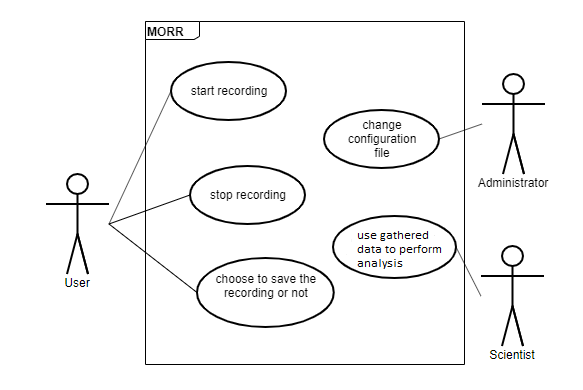
\includegraphics[scale=0.9]{resources/usecase.png}
\end{center}     % Scenarios
\chapter{Systemmodels}
\label{ch:sysmodels}

\section{System architecture}
\label{sec:sysarchitecture}
The specified criteria demand for a minimalist user interface and little to no bidirectional data flow within the application. As the main focus of this project is collecting, processing and finally storing data, the applied architecture will be a pipeline architecture.

\subsection{Basic Pipeline}
\label{sec:sm_basicpipe}
The traditional pipeline architecture refers to a process being split up into several sequential steps, ideally with data buffers in between those, which will be able to independently and possibly asynchronously perform a specific transformation on their data input. The resulting data will then be provided as output for the subsequent step. This works especially well in a scenario where only an unidirectional data flow is required.
\begin{figure}[h!]
  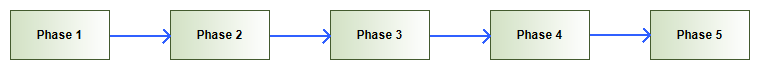
\includegraphics[width=1.00\textwidth]{resources/simplepipeline.png}
  \centering
  \caption{A simple pipeline model}
  \label{fig:sm_basicpipe}
\end{figure}

\subsection{The extended pipeline}
\label{sec:sm_extpipe}
In this project, the basic pipeline is an insufficient model, as the initial input data will have to be gathered at several, mostly independent places. The \gls{browser} module (see \specref{FS440} to \specref{FS449}) will only capture \gls{browser} \glspl{event}, the window management \gls{module} (see \specref{FS400} to \specref{FS404}) cannot also provide the keyboard input etc. In order to solidify all the collected \glspl{event}, the extended pipeline allows for a single processing step to accept input from multiple sources by utilizing the transforming modules as mentioned in \ref{transforming-module}. The result is a tree-structure where the \gls{event}-data strictly flows from the leafs towards the root, the root being the core application (see \ref{sec:func_core}).
\begin{figure}[h!]
  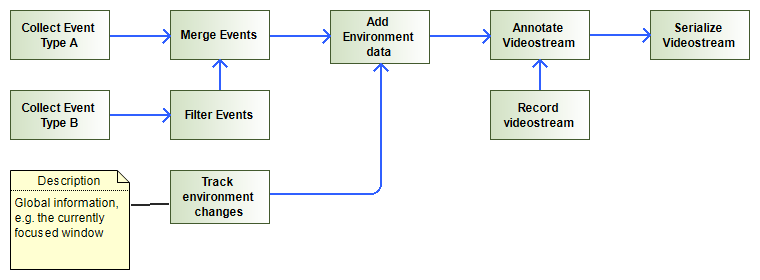
\includegraphics[width=1.00\textwidth]{resources/extendedpipeline.png}
  \centering
  \caption{An extended pipeline model}
  \label{fig:sm_extpipe}
\end{figure}

\subsection{Module types}
\label{sec:module-types}


The application needs to provide three different types of \glspl{module}:
\begin{itemize}
        \item Collecting \glspl{module}\label{collecting-module}\\\Glspl{module} which accept no input from other \glspl{module} and generate one or more \glspl{event} as output.
        \item Transforming \glspl{module}\label{transforming-module}\\\Glspl{module} which accept one or more \glspl{event} as input from other \glspl{module} and generate one or more \glspl{event} as output.
        \item Discarding \glspl{module}\label{discarding-module}\\\Glspl{module} which accept one or more \glspl{event} as input from other \glspl{module} and output no \glspl{event}.
\end{itemize}

%\section{Object models}
%%we might not want to specify object models yet

\newpage %%formatting, can potentially be removed later
\section{Dynamic model} %%change to models should addtional charts be added
\label{sec:sm_dynamic_models}
The following figure shows an example of how the application could deal with a \gls{user} clicking on an element in their \gls{browser}. The actual flow might differ based on available modules and rule configuration.
\begin{figure}[H]
  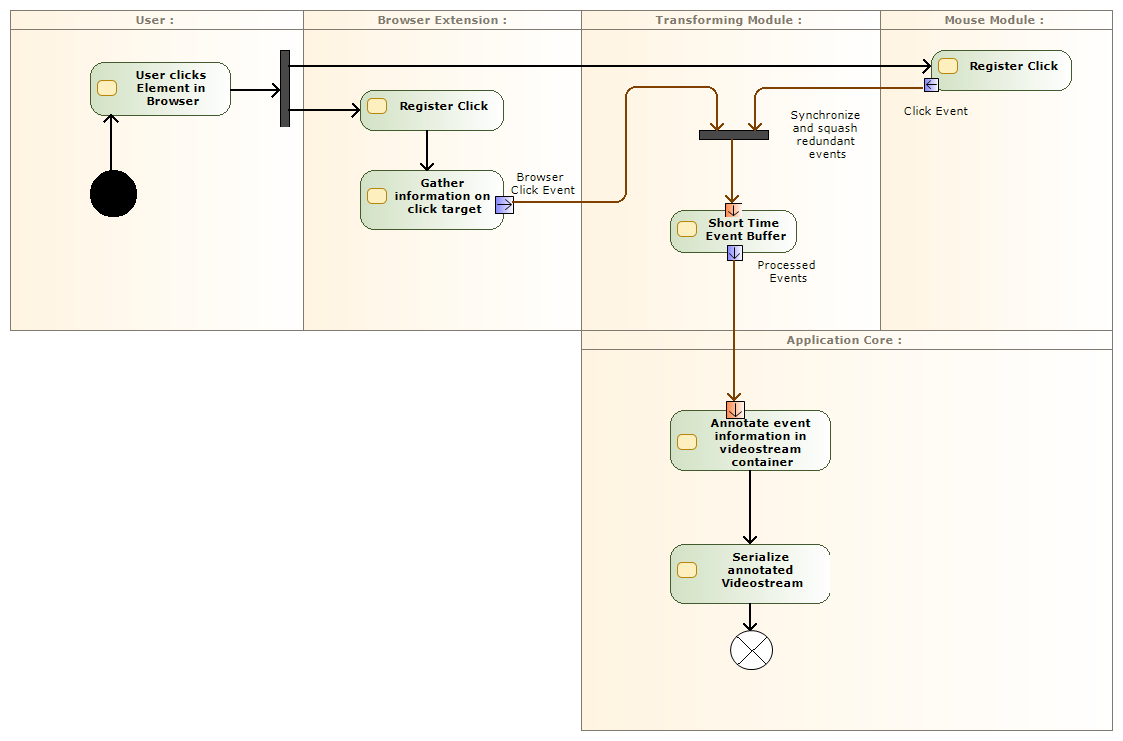
\includegraphics[width=1.00\textwidth]{resources/clickactivity.png}
  \centering
  \caption{User-Click sample activity chart}
  \label{fig:sm_clickactivity}
\end{figure}
\newpage %% for formatting
\section{User Interface}
\label{sec:sm_userinterface}
The \gls{user}-interface is intentionally minimal as the \glspl{user} should not be disrupted during their usual work-routine. The following figures show drafts and therefore do not represent the final product.

\begin{figure}[H]
  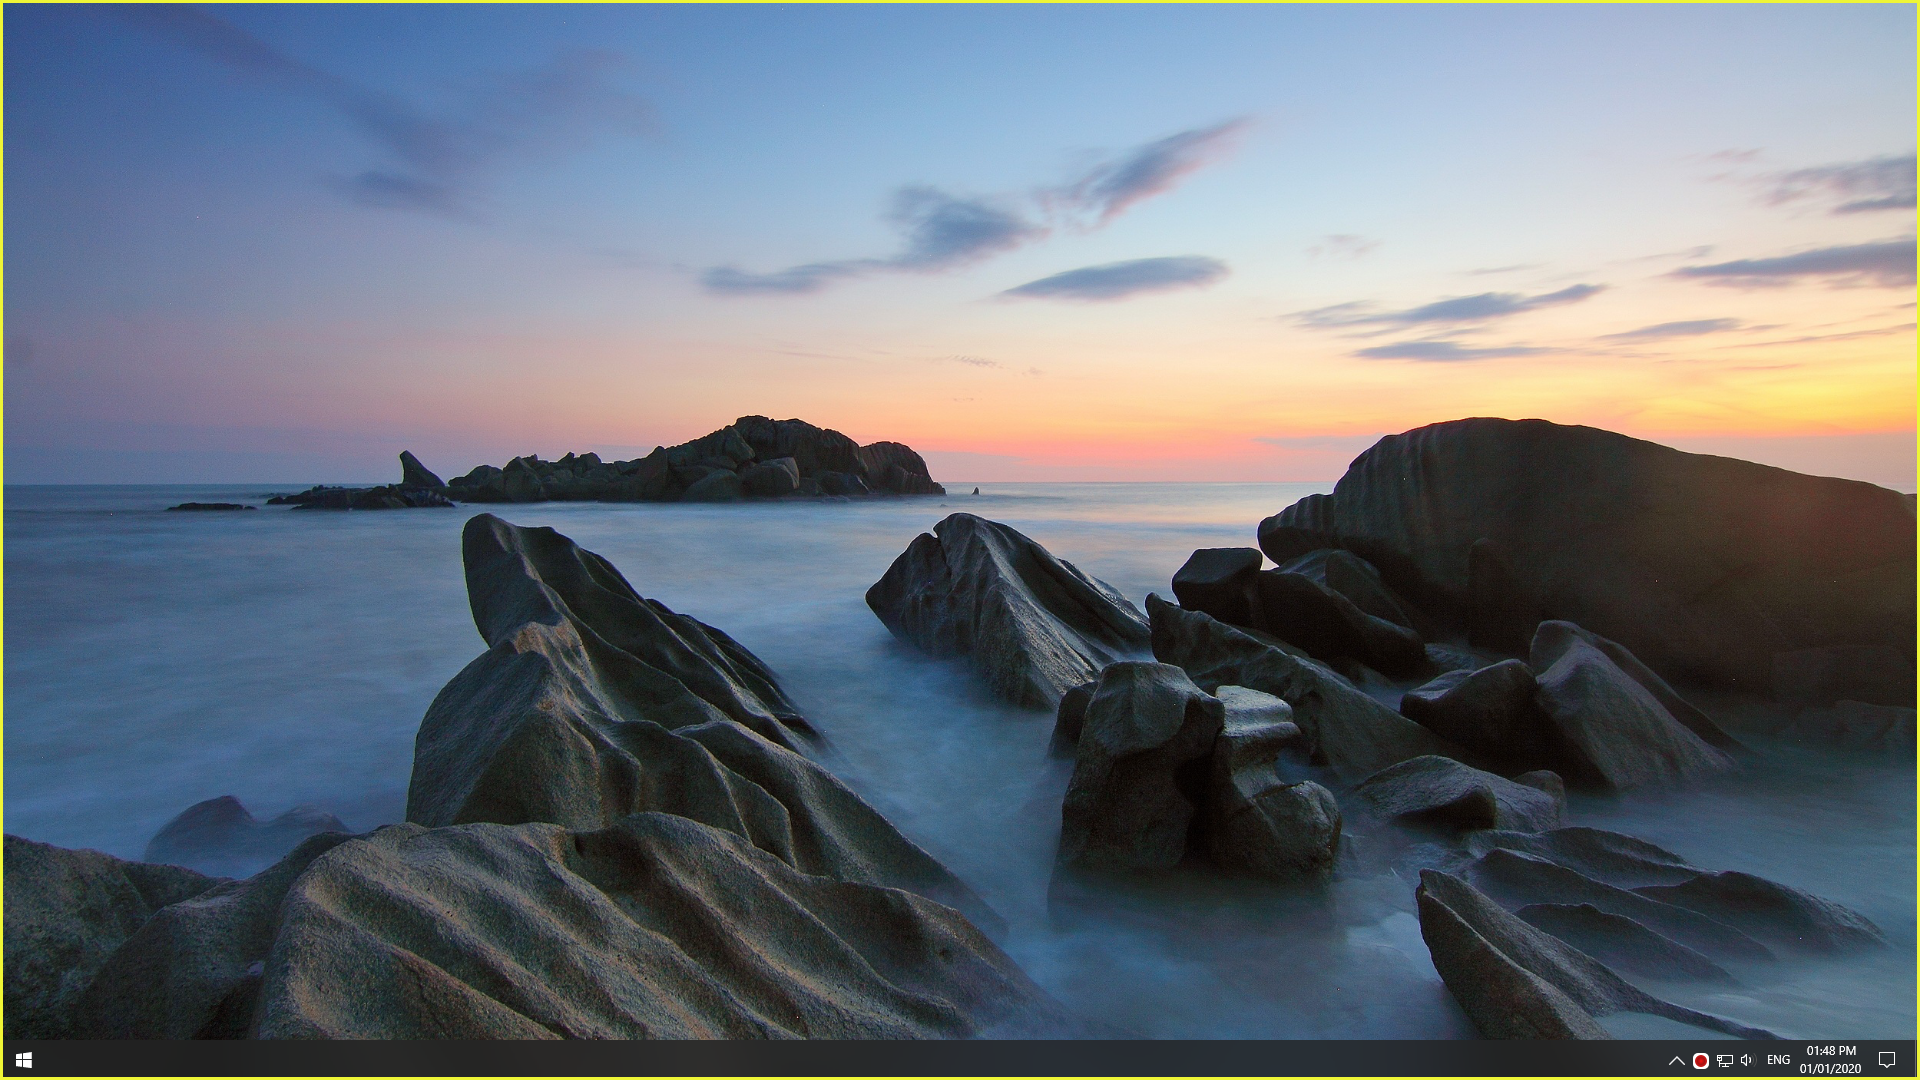
\includegraphics[width=1.00\textwidth]{resources/ui_recording.png}
  \centering
  \caption{A running \gls{session} recording is indicated by a yellow border.}
  \label{fig:sm_ui_recordindicator}
\end{figure}
\begin{figure}[H]
  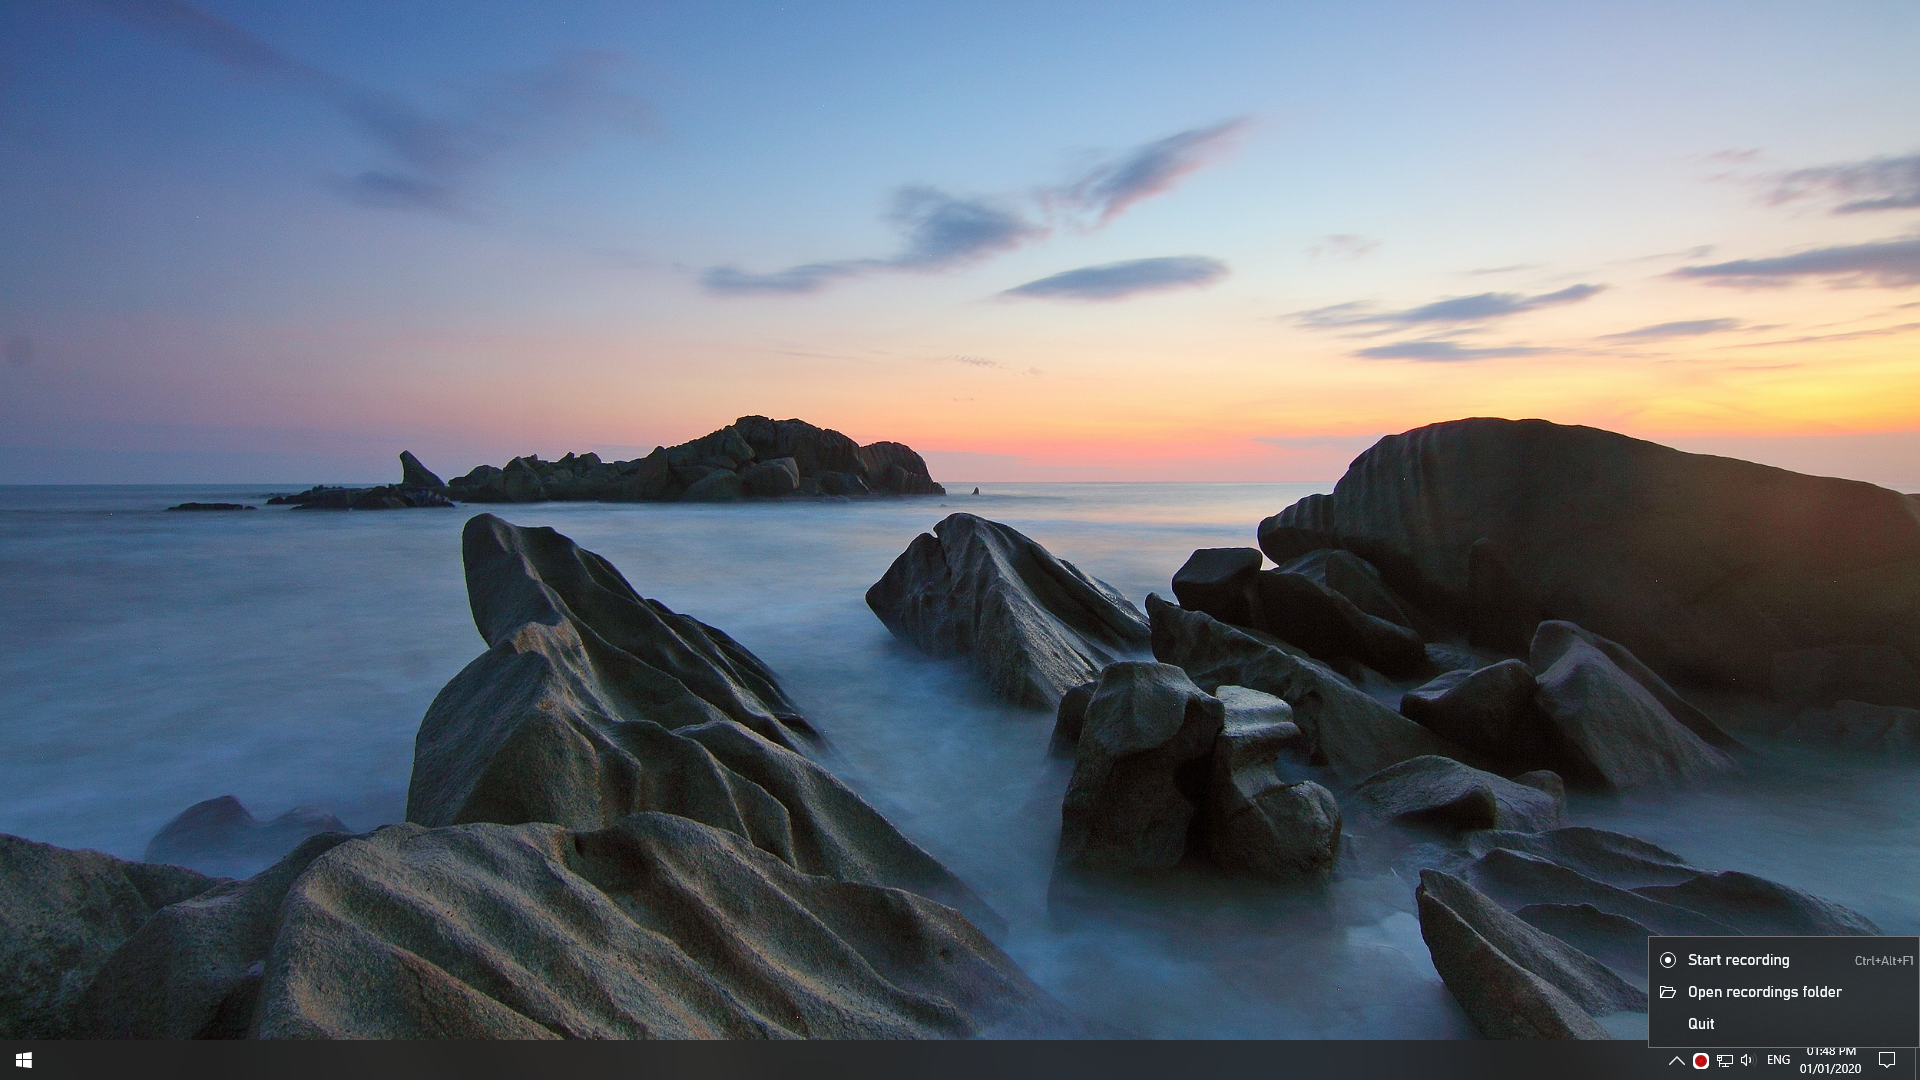
\includegraphics[width=0.5\textwidth, trim={50cm 0 0 25cm},clip]{resources/ui_inactive_tray.png}
  \centering
  \caption{The start/stop recording features may be quickly accessed by clicking on the tray icon (represented by the red dot).}
  \label{fig:sm_ui_trayicon}
\end{figure}
\begin{figure}[H]
  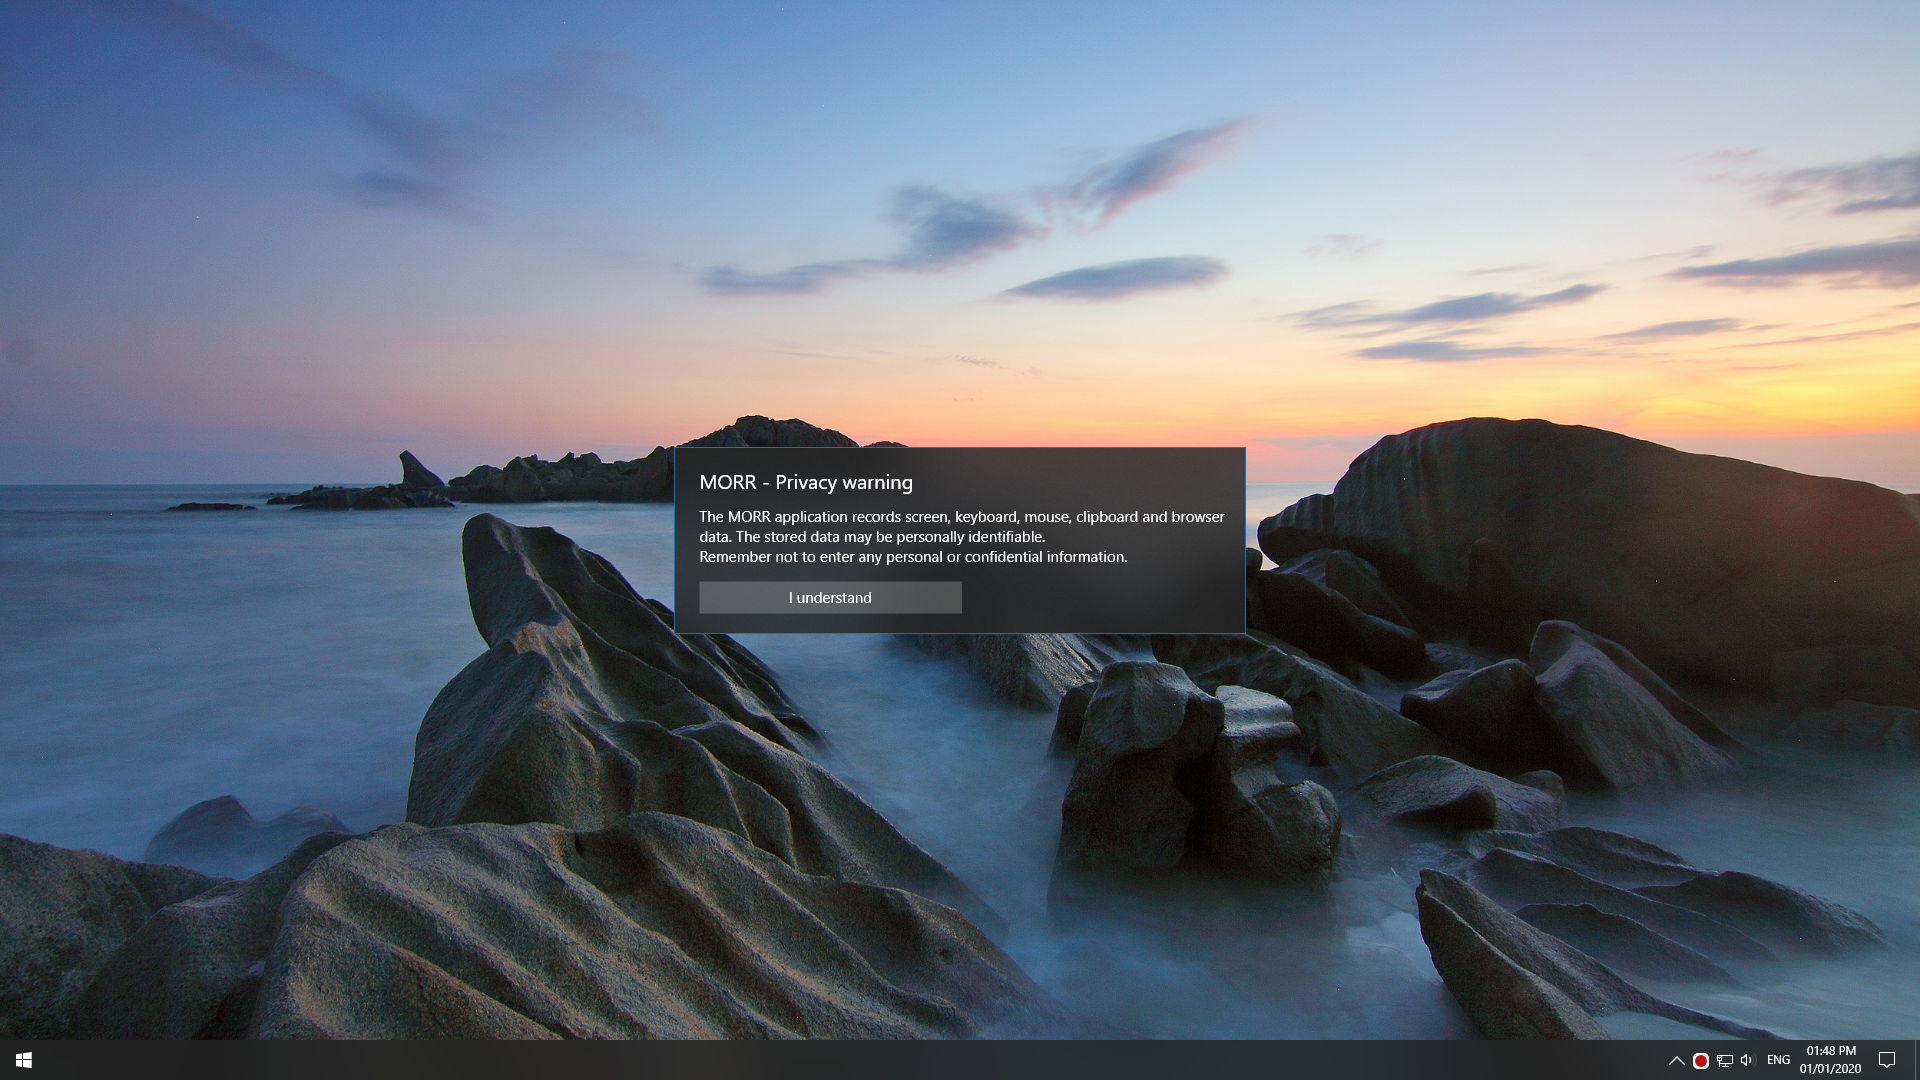
\includegraphics[width=0.8\textwidth, trim={20cm 10cm 20cm 10cm}, clip]{resources/ui_privacy_warning.png}
  \centering
  \caption{The privacy warning appears when a recording is started.}
  \label{fig:sm_ui_privacy}
\end{figure}
\begin{figure}[H]
  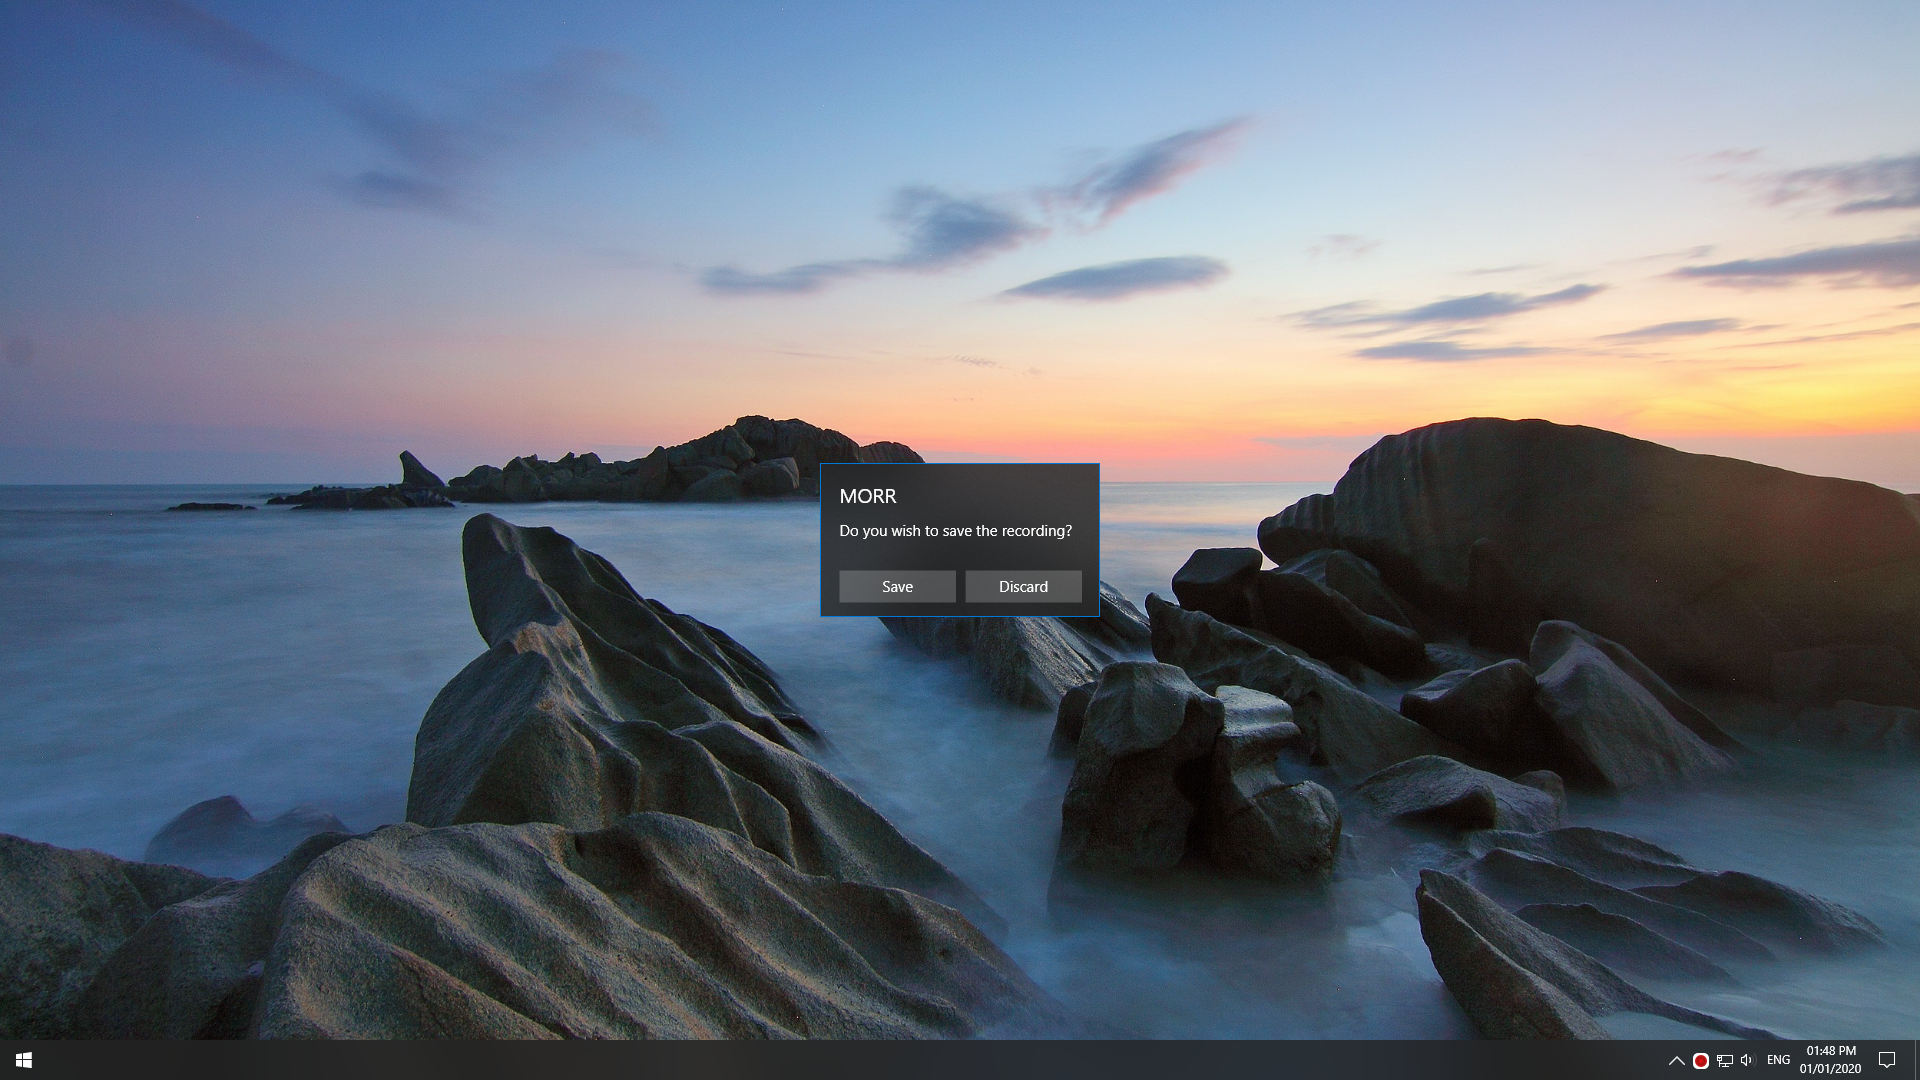
\includegraphics[width=0.8\textwidth, trim={20cm 10cm 20cm 10cm}, clip]{resources/ui_save_dialogue.png}
  \centering
  \caption{The save dialogue appears when a recording is stopped.}
  \label{fig:sm_ui_saving}
\end{figure}

\subsection{Data extraction}
\label{sec:sm_extraction}
The \glspl{scientist} will be able to extract \gls{event}-information from the videocontainer by utilizing an API (application programming interface) which will be supplied together with the application. Additionally, the application will be bundled with a commandline-tool which allows for extraction of the \gls{event}-data into the common CSV-format (comma-separated values). See also \specref{FS330}.		% System Models
\chapter{Feasibility Study}
\label{ch:feasibility}

\section{Alternatives}
\section{Technical Feasibility}
\section{Personnel Feasibility}
\section{Risks}
\section{Economical Feasibility}
\section{Legal Feasibility}
 	% Feasibility Study
\printnoidxglossaries
\end{document}
